
\normalsize
\section{Porous Medium Properties}

\begin{verbatim}
#SOIL_PROPERTIES
\end{verbatim}

\subsection{Current Status}

Currently the soil properties are entered either by using a key
word which starts with a \verb+#+ sign and then a whole series of
input values in the order presented in table 1, (old method) or
increasingly by a more easy to comprehend key word which starts
with a \verb+$+ sign, and then the required values follow. A
description of the models and the input parameters can be found in
the following sections.

\vspace{0.5cm}

In summary the following \verb+$+ key words have been implemented
to date:-

\begin{verbatim}

$CAP_PRESSURE_SATURATION
$ELECTRIC_CONDUCTIVITY
$FLUID_EXCHANGE_WITH_OTHER_CONTINUA
$FLUID_STORATIVITY
$NAME
$REL_PERMEABILITY_DEFORMATION
$REL_PERMEABILITY_SATURATION
$REL_PERMEABILITY_PRESSURE
$REL_PERMEABILITY_VELOCITY
$UNCONFINED_FLOW_GROUP

\end{verbatim}


%\setlength{\evensidemargin}{-1.0cm}


%beginning of table region

\begin{table}[htbp]

\begin{center}

\footnotesize

\begin{tabular}{|c|l|c|l|c|c|}

\multicolumn{6}{c} {\textbf{Table 1: Soil Properties}}  \\
\hline
Param & RF variable / \$Keyword & Value & Meaning &No. Mod.&Unit\\
 &   &  &  &Par.&Unit\\

\hline \hline
N1    & dimension & 1 & Element dimension & 1 N1a &[-]\\
      &           & 2 &                   & 1 N1a&[-]\\
      &           & 3 &                   & 0 &   \\
\hline
N1a   & area      & 1 & Element exchange area (1D) &1 &[m$^{2}$]\\
      &           &   & Element thickness (2D) & 1&[m]\\
\hline

N2    & porosity model& 0 & Constant value & [-]&[-]\\
      &               & 1 & Solution dependent & 6 (see text)& [-]\\
      &               & 2 & Swelling dependent & 5 (see text)& [-]\\
\hline

N3    & tortuosity    & 1 & Medium tortousity &1& [-]\\
\hline

N4    & .number\_grain\_classes &0& &[-]&[-]\\
    &   &1&No. of lithological
components & [No.]& [-]\\
N4a X No.    &   &&Grain class radius &X No.&[m]\\
N4b X No.    &   &&Grain class percentage &X No.&[\%]\\
\hline

N5 & .nonlinearflowelement&0&- Linear flow&[-]&[-]\\
   &                      &1&- Non linear &1 [$\gamma$]&[-]\\
\hline

N6 & .storativity &0&Constant value&1&[m]\\
  & \$FLUID\_STORATIVITY &0&Constant value &1& \\
   & \$FLUID\_STORATIVITY &1&Over curve (see text) &1& \\
  & \$FLUID\_STORATIVITY &2& (see text) &4& \\
  & \$FLUID\_STORATIVITY &3& (see text) &3& \\
  & \$FLUID\_STORATIVITY &4& (see text) &3& \\

\hline

N7& .permeabilitymodel &0& Isotropic permeability &1&[m$^{2}$]\\
&&&(1D, 2D, 3D)&&\\
&permeabilitytensor&1& Perm. tensor (2D )&4&\\
&k[ ]&&k$_x$$_x$ k$_x$$_y$ k$_y$$_x$ k$_y$$_y$&&[m$^{2}$]\\
&&1& Perm. tensor (3D )&9&\\
&k[ ]&&k$_x$$_x$ k$_x$$_y$ k$_x$$_z$ &&[m$^{2}$]\\
&&&k$_y$$_x$ k$_y$$_y$ k$_y$$_z$ &&[m$^{2}$]\\
&&&k$_z$$_x$ k$_z$$_y$ k$_z$$_z$ &&[m$^{2}$]\\
&&3& Perm. distribution (see text)&&\\

\hline

N8& .perm[ ]& &Permeability f(S) relationships&6&\\
&\$REL\_PERMEABILITY&& (see text)&&\\
&\_SATURATION&&Models 1,2,3,4,5,6,7,8,11,12,13&&\\
 \hline

N9& .kap[ ]&1 to 11&Capillary pressure functions&5&\\
&\$CAP\_PRESSURE&& (see text)&&\\
&\_SATURATION&&Models 1,2,3,4,5,6,7,11&&\\
\hline

N10& .massdispL&(value)&Longitudinal mass &&\\
&&&dispersion length&&[m]\\
\hline

N11& .massdispT&(value)&Transverse mass&&\\
&&&dispersion length&&[m]\\

\hline

N12& .heatdispL&(value)&Longitudinal heat &&\\
&&&dispersion length&&[m]\\

\hline

N13& .heatdispT&(value)&Transverse heat&&\\
&&&dispersion length&&[m]\\

\hline

N14&.heatconductivitymodel&0& isotropic heat conductivity   & 1& [Wm$^{-1}$K$^{-1}$] \\
   &.heatconductivitytensor[ ]& & && \\
       &                               &   1     & 2D 2 Values $\lambda$ $_x$$_x$ $\lambda$ $_y$$_y$&2&[Wm$^{-1}$K$^{-1}$]\\
       &                               &    1    & 3D 3 Values $\lambda$ $_x$$_x$ $\lambda$ $_y$$_y$ $\lambda$ $_z$$_z$&3&[Wm$^{-1}$K$^{-1}$]\\
\hline

N15&.densityrock&(value)&Rock density&1&[Kgm$^{-3}$]\\

\hline

N16&.heatcapacityrock&(value)&Heat capacity of soil or rock &1&[JKg$^{-1}$K$^{-1}$]\\


\hline

\end{tabular}
\end{center}
\end{table}

%}%End of table region
\normalsize
\newpage

\subsection{Description of input sequences.}

\textbf{Data Input - MAT-MP}

\vspace{0.5cm}

\textbf{N1  Element Dimension}
\begin{center}
\begin{tabular}{l|l}
%
Dimension & Extra value required \\
\hline
1 & Element exchange area \\
2 & Element thickness \\
3 & No value accepted
\end{tabular}

\end{center}
%\end{center}


\vspace{0.5cm}

\vspace{0.5cm}

\textbf{Example}
\newline

\#SOIL\_PROPERTIES..

 2 1 ; Dimension, value

\vspace{0.5cm}

\textbf{N2  Porosity Models}

Porosity models describe the porosity changes in the porous media.
There are three classes of model:-

\vspace{0.5cm}
\begin{center}
\begin{tabular}{l|l}
Model & \\
\hline
%
0 & constant value \\
%
1 & 0 constant value  \\
  & 1 porosity changes by salt dissolution  \\
%
2 & porosity changes by swelling\\
\end{tabular}
\end{center}
\vspace{0.5cm}
\textbf{Example}
\begin{verbatim}
#SOIL_PROPERTIES ..
 0 0.2 ; porosity model, porosity value (0 to 1)
\end{verbatim}

\textbf{Model 1:   Salt dissolution model}

\vspace{0.5cm}

\begin{eqnarray}
n=\frac{n+2n*dis*b*{\DensSolid}*({\Solubility}-a)*dt}{\DensSolid}
\end{eqnarray}

\begin{tabular}{l|l}
Value & Physical Meaning\\
\hline
%
$\DensSolid$ & Density of Solid Material \\
$\DensFluid$ & Density of Fluid Material  \\
$\Solubility$ & Solubility Coefficient  \\
dis & Dissolution Rate \\
a & Fist input parameter to model \\
b & Second input parameter to model \\
\end{tabular}

\vspace{0.5cm}

\textbf{SubModel:   B\"{o}rgesson Swelling Model}

\vspace{0.5cm}

B\"{o}rgesson Swelling Model can be activated by adding the sub-key
words \\ \$REL\_PERMEABILITY\_DEFORMATION" under the key words \#
SOIL\_PROPERTIES". One example is:

\footnotesize

\begin{verbatim}
#SOIL_PROPERTIES ...

$REL_PERMEABILITY_DEFORMATION  ;B\"{o}rgesson swelling model ;model
k0  eps0 eta   p^sw_0     beta   p^sw as curve
     1  1.0 1.0  4.640 1e7       -0.187 2.00  ; Swelling pressure
  N1    N2   N3   N4    N5        N6     N7

#CURVES ;curve No. 2.00 ;S^W  P^sw[Pa]
 0.6 1e7 ; initial saturation
 0.7 4e7
 1.0 5e7
\end{verbatim}

\normalsize
\begin{tabular}{|c|c|c|l|c|c|}
\hline
\multicolumn{6}{|c|} {B\"{o}rgesson Swelling Model} \label{Tab:Boergesson} \\
\hline
Param. & RF variable              & Value & Description                         &  Equation              & Unit  \\[0.5ex]
\hline \hline
N1     & .swelling\_model         & 0      & without swelling model              &                       &  $[-]$   \\
       &                          & 1      & B\"{o}rgesson swelling model            &                       &          \\
\hline
N2     & .rel\_perm\_defo\_val[0] & double & Relative permeability $k_{rel0}^\varepsilon$ & (\ref{eqn:relPer}) & $[m^2]$ \\
N3     & .rel\_perm\_defo\_val[1] & double & void ratio $e_0$                    & (\ref{eqn:voidRatio})  &  $[-]$  \\
N4     & .rel\_perm\_defo\_val[2] & double & eta $\eta$                          & (\ref{eqn:eta})        &  $[-]$  \\
N5     & .rel\_perm\_defo\_val[3] & double & Swelling Pressure $p^{sw}_0$        & (\ref{eqn:SwellPress}) &  $[-]$  \\
N6     & .rel\_perm\_defo\_val[4] & double & beta $\beta$                        & (\ref{eqn:beta})       &  $[-]$  \\
N7     &                          & double & Relation of swelling pressure       &                        &          \\
       &                          &        &  with saturation in curve           &                        &          \\
\hline
\end{tabular}
\\
\begin{eqnarray}
k^\varepsilon_{rel}(p(S^W)) =
k^\varepsilon_{rel0}\left(\frac{e(p(S^W))}{e_0}\right)^\eta
\label{eqn:relPer}
\end{eqnarray}

\begin{eqnarray}
e=\frac{1}{1-n} \label{eqn:voidRatio}
\end{eqnarray}

\begin{eqnarray}
\eta = \frac {\Delta(\mathrm{ln~}{k^\varepsilon_{rel}})}
{\Delta(\mathrm{ln~} e)} \quad , \quad 0.5 < e < 2 \label{eqn:eta}
\end{eqnarray}

\begin{eqnarray}
e(p(S^W))=e_0 \left( \frac{p(S^W}{p_0}\right)^\beta
\label{eqn:SwellPress}
\end{eqnarray}

\begin{eqnarray}
\beta = \frac{\Delta ln e}{\Delta ln p(S^W)}<0 \label{eqn:beta}
\end{eqnarray}


\textbf{SubModel: CSM Swelling Model}

\vspace{0.5cm}

CSM Swelling Model can be activated by adding the sub-key words
"\$REL\_ PERMEABILITY\_ DEFORMATION" under the key words "\#
SOIL\_PROPERTIES". One example is:

\footnotesize

\begin{verbatim}
#SOIL_PROPERTIES ...

$REL_PERMEABILITY_DEFORMATION ;CSM swelling model

;model  k0  eps0   eta     beta
  2     1.0 1.01   4.640   -0.187
  N1    N2   N3    N4      N5
\end{verbatim}

This model calculate the relative permeability using the effective
porosity according to the CSM model (Xie et al. 2003). It is
suitable for expansive soil material like bentonite or
bentonite/sand mixtures.

The meaning of the parameters $k0$, $eps0$, $eta$ and $beta$ are
the same as those described in the B\"{o}rgesson model mentioned above
(Table \ref{Tab:Boergesson}). The governing equations for the
calculation are:

\begin{eqnarray}
k^\varepsilon_{rel}(n_{eff})) =
k^\varepsilon_{rel0}\left(\frac{e(n_{eff})}{e_0}\right)^\eta
\label{eqn:relPerCSM}
\end{eqnarray}

\begin{eqnarray}
e=\frac{1}{1-n_{eff}} \label{eqn:voidRatioCSM}
\end{eqnarray}

\normalsize

\textbf{N3  Tortuosity} \vspace{0.5cm}

This is a single value representing the tortousity of the solid
material. To date there are no tortousity models implemented in
the RockFlow code.

Example

1  Value of Tortousity

\vspace{0.5cm}

\textbf{N4  Lithology} \vspace{0.5cm}


\begin{tabular}{l|l}
Model & \\
\hline
%
0 & not active \\
1   & .number\_grain\_classes\\
    &No. of lithological components\\
    &Grain class radius\\
    &Grain class percentage\\
\end{tabular}
\vspace{0.5cm}

\textbf{N5  Flow Model}

\begin{tabular}{l|l}
Model & Physical Meaning\\
\hline
%
0 & Linear Flow, no extra parameter required \\
1 & Non Linear Flow, parameter $\gamma$ required  \\

\end{tabular}

\vspace{0.5cm}

For non-linear flow the hydraulic conductivity is given
by:\index{material - hydraulic conductivity}
\begin{eqnarray}
{\bf K} (\nabla h) &=& {\bf K}_0 \mid\nabla h \mid^{\gamma -1} =
{\bf K}_0 K_{\mbox{\footnotesize rel}}
\\[3pt]
\gamma &=& \left\lbrace
\begin{array}{ll}
> 1 & \mbox{pre-linear}
\\
= 1 & \mbox{linear (Darcy law)}
\\
< 1 & \mbox{post-linear}
\\
    & = 1/2 \mbox{ turbulent friction}
\end{array}
\right.
\end{eqnarray}

The non-linear flow parameter $\gamma$ divides three flow regimes:
pre-linear, linear, and post-linear ones. In the pre-linear modus,
motion is restricted by electro-molecular forces attracting the
fluid molecules to the solid surface. The pre-linear regime is
characterized by small pressure gradients $|\nabla h|\ll 1$,
whereas the post-linear regime is characterized by large gradients
$|\nabla h|\gg 1$. In the post-linear mode, motion is restricted
by non-linear friction effects. From the above equation it can be
seen, the effective hydraulic resistance $K_{\mbox{\footnotesize
rel}}$ increases for smaller pressure gradients in pre-linear
situations and for larger pressure gradients in post-linear
situations as well.

\vspace{5mm}

\textbf{N6  Storage}

\vspace{0.5cm}

 Storativity of the porous medium

\vspace{0.5cm}

\begin{tabular}{l|l}
%
Model & \\
\hline
%
0 & constant value N1 \\
1 & values defined by a \#CURVE as a function of fluid pressure $\FluidPressure$\\
2 & Function of pressure from the middle of the element, N1, N2, N3, N4\\
3 & Function of pressure from the middle of the element, N1, N2, N3, N4\\
4 & values defined by a \#CURVE as a function of effective stress, N1, N2, N3 \\

\end{tabular}
%\end{center}

\vspace{0.5cm}

Input Parameters for the Models

\vspace{0.5cm}
\begin{tabular}{l|l}
%
Model & \\
\hline
%

2 & $\sigma'$=$\frac{N3+N4}{2}$-$\FluidPressure$\\
  &  \\
  & $\Stor$=N1-N2(Log$\sigma'$)\\
  &  \\
3 & $\sigma'$=$\frac{N1+N2}{2}$-$\FluidPressure$\\
  &  \\
  & values defined by a \#CURVE as a function of $\sigma'$ calculated as shown\\
  & N1 : Curve Number\\
4 & $\sigma'$=$\sigma$-$\FluidPressure$\\
  & N1 : Curve Number \\
  & N2 : Time Collation Factor (0.5)\\
  & N3 : Rock Density\\
  & values defined by a \#CURVE as a function of $\sigma'$ calculated as shown\\

\end{tabular}
%\end{center}

\vspace{0.5cm}

\textbf{Example}

\begin{verbatim}

$FLUID_STORATIVITY

4 2.0 0.5 2800.0 ; model, Curve Number, Time Collation Factor,
Rock Density
\end{verbatim}
\vspace{0.5cm}

\textbf{N7  Permeability}
\vspace{0.5cm}

It is possible to specify permeability in 1D, 2D and 3D as a
single isotropic value, an anisotropic value, a function of
fracture roughness (2D fracture only), and as a function of
saturation.

\begin{tabular}{|c|c|c|l|}
\hline
\multicolumn{4}{|c|} {Permeability Models} \label{Tab:Boergesson} \\
\hline
Model  & RF variable              & Value & Meaning                        \\[0.5ex]
\hline \hline
0 0    & isotropic permeability  & (Value) & One value in all directions \\
0 1    & anisotropic permeability & double & Number of input value depends on the dimension \\
       &                          &        & 2D 2 Values kxx kyy\\
       &                          &        & 3D 3 Values kxx kyy kzz\\
0 3    & distribution & & See comment below\\
\hline
\end{tabular}
\vspace{0.5cm} \vspace{0.5cm}

It is possible to introduce a permeability distribution. This
option is currently activated for 2D fractures. The permeability
of each element is calculated according to the cubic law. For this
purpose the key word \verb+#FRACTURE-APERTURE_DISTRIBUTION+ has to
be used which defines the fracture aperture for each element.
(Ordering is by element number.)

Example

0 3 ;Permebility model, tensor type

\begin{verbatim}
#FRACTURE_APERTURE_DISTRIBUTION
\end{verbatim}

\begin{tabular}{c c c c}

1.4136E-05  &   6.8681E-05  &   5.3747E-05  &   4.9235E-05\\
4.9631e-05  &   1.2517E-05  &   2.0050E-06  &   7.9725E-05\\
2.4056E-05  &   8.8494E-05  &   2.3222E-05  &   6.0452E-05\\
6.7105E-05  &   4.3951E-05  &   7.0117E-05  &   1.8700E-05\\
6.1989E-05  &   3.6385E-05  &   2.0621E-05  &   5.9200E-05\\
3.8982E-05  &   7.8354E-05  &   4.0144E-05  &   6.5515E-05\\
3.7302E-05  &   4.2645E-05  &   2.7392E-05  &   5.4282E-05\\
\end{tabular}

\vspace{0.5cm}

Number of elements........

\vspace{0.5cm}
\newpage
\textbf{N8  Permeability as a function of saturation }

\vspace{0.5cm}


Numerous relationships between relative permeability and
saturation are given in the literature. We list some of the most
common which are implemented in the Rockflow code.

% Tabelle als Gleitumgebung
\footnotesize
\begin{table}[htb!]
\caption{Rockflow models} \label{tab:} \vspace{-3mm}
\begin{center}
\begin{tabular}{|ll|llllll|}
\hline
      & $\PermRelS(\Saturation)$ model & & & & & &\\
\hline
rp[0] &                     & rp[1] & rp[2] & rp[3] & rp[4] & rp[5] & rp[6]\\
\hline
0 & Perfectly mobile phases &  &  &  &  &  & \\
\hline
1 & User-defined curve      & 1st & 2nd & ... & & & \\
\hline
2 & Linear function         & $\Saturation^g_1$ & $\Saturation^g_2$ &  & $\Saturation^w_1$ & $\Saturation^w_2$ & \\
\hline
3 & Parabolic function      & $\Saturation^g_1$ & $\Saturation^g_2$ & a & $\Saturation^w_1$ & $\Saturation^w_2$ & b \\
\hline
4 & van Genuchten (1980)    & $\SaturationRes^w$ & $\SaturationMax^w$ & $\alpha$ & m & n & \\
&Burdine's Equation&&&&&&\\
\hline
5 & Haverkamp et al. (1977) & $\SaturationRes^w$ & $\SaturationMax^w$ & $\alpha$ & A & $\beta$ & \\
\hline
6 & Brooks \& Corey   & $\SaturationRes^w$ & $\SaturationMax^w$ &  &  &  & \\
 & (simple) (1966)  & & &  &  &  & \\
\hline
7 & Jump function  & & &  &  &  & \\
\hline
8 & Brooks \& Corey (1966)  & $\SaturationRes^w$ & $\SaturationMax^w$ & Pore size Dist.&  &  & \\
\hline
11 & Three phases & Curve No. & Curve No. & Curve No.  &  &  & \\
 & over curves & & & &  &  & \\
\hline
12 & Three phases, & $\Saturation^g_1$ & $\Saturation^g_2$ & a & $\Saturation^w_1$ & $\Saturation^w_2$ & b \\
& nonlinear relationship & &&& &&\\
\hline
13 & van Genuchten (1980)&   $\SaturationRes^w$ & $\SaturationMax^w$ & $\alpha$ & m & n & \\
&Mualems Equation&&&&&&\\
 \hline
\end{tabular}
\end{center}
\end{table}
%
\normalsize

\vspace{-5mm} Rockflow functions:

\texttt{void CECalcRelPerm\_AMM(long element,int phasen,double
*satu,double *relperm)}

%-------------------------------------------------------------------------------

\vspace{5mm}

\textbf{0 - Perfect mobile phases}
\begin{eqnarray}
\PermRelS^g = 1 \quad , \quad \PermRelS^w = 1
\end{eqnarray}

%-------------------------------------------------------------------------------
\textbf{1 - User-defined function}
\begin{eqnarray}
\PermRelS^g = f(\Saturation^g_i) \quad , \quad \PermRelS^w =
f(\Saturation^w_i)
\end{eqnarray}

%-------------------------------------------------------------------------------
\textbf{2 - Linear function}
\begin{eqnarray}
\PermRelS^g &=& \left\{
\begin{array}{ll}
0 & \Saturation^g < \Saturation^g_1
\\
\D\frac{\Saturation^g-\Saturation^g_1}{\Saturation^g_2-\Saturation^g_1}
& \Saturation^g_1 < \Saturation^g < \Saturation^g_2
\\
1 & \Saturation^g > \Saturation^g_2
\end{array}
\right.
\\
\PermRelS^w &=& \left\{
\begin{array}{ll}
0 & \Saturation^w < \Saturation^w_1
\\
\D\frac{\Saturation^w-\Saturation^w_1}{\Saturation^w_2-\Saturation^w_1}
& \Saturation^w_1 < \Saturation^w < \Saturation^w_2
\\
1 & \Saturation^w > \Saturation^w_2
\end{array}
\right.
\end{eqnarray}


%-------------------------------------------------------------------------------
\textbf{3 - Potential function}
\begin{eqnarray}
\PermRelS^g &=& \left\{
\begin{array}{ll}
0 & \Saturation^g < \Saturation^g_1
\\
\left(
\D\frac{\Saturation^g-\Saturation^g_1}{\Saturation^g_2-\Saturation^g_1}
\right)^a & \Saturation^g_1 < \Saturation^g < \Saturation^g_2
\\
1 & \Saturation^g > \Saturation^g_2
\end{array}
\right.
\\
\PermRelS^w &=& \left\{
\begin{array}{ll}
0 & \Saturation^w < \Saturation^w_1
\\
\left(
\D\frac{\Saturation^w-\Saturation^w_1}{\Saturation^w_2-\Saturation^w_1}
\right)^a & \Saturation^w_1 < \Saturation^w < \Saturation^w_2
\\
1 & \Saturation^w > \Saturation^w_2
\end{array}
\right.
\end{eqnarray}


Such a function was introduced e.g. by Huyakorn \& Pinder (1983).
\begin{eqnarray}
\PermRelS^w = \frac{(\Saturation^w-0.2)^2}{0.36}
\end{eqnarray}

%-------------------------------------------------------------------------------
\textbf{4 - van Genuchten Model (1980)}
\begin{eqnarray}
\PermRelS(h) = \frac{1-(\alpha h)^{n-2}\,[1+(\alpha
h)^n]^{-m}}{[1+(\alpha h)^n]^{2m}}
\end{eqnarray}

% *** EPS-Grafik ***
\begin{figure}[htb!]
\begin{center}
\footnotesize
%\psfrag{Synonym}[pos][pos]{Tex-Ersetzung}
%\psfrag{x}[][]{$t$}
%\psfrag{y}[b][t]{$y(t)$}
%\psfrag{t}[][]{ }
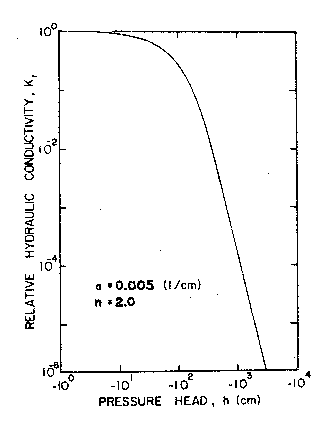
\includegraphics[width=0.5\columnwidth]{F:/Rockflow/New_manual/Chapter15/figures/van_gen1.eps}  % Filename.eps
\caption{Relative permeability functions (Source: van Genuchten
Model (1980))} \label{fig:}
\end{center}
\end{figure}
%


%-------------------------------------------------------------------------------
\textbf{5 - Haverkamp et al. (1977)}
\begin{eqnarray}
\PermRelS(h) = K_s \frac{A}{A+|h|^\beta}
\end{eqnarray}
\begin{eqnarray}
h = \left( -\frac{\alpha}{\theta} (\theta - \theta_s + \theta_r)
\right)^{1/\beta}
\end{eqnarray}



%-------------------------------------------------------------------------------
\textbf{6 - Brooks \& Corey (1966)Simple}
\begin{eqnarray}
\SaturationEff =
\frac{\Saturation^w-\SaturationRes^w}{\SaturationMax^w-\SaturationRes^w}
\end{eqnarray}
\begin{eqnarray}
\PermRelS^w = \SaturationEff^4
\end{eqnarray}

%-------------------------------------------------------------------------------
\textbf{7 - Jump Function} \vspace{5mm}

%-------------------------------------------------------------------------------
\textbf{8 - Brooks \& Corey (1966)} \vspace{5mm}

%-------------------------------------------------------------------------------
\textbf{11 - Three phases over curves} \vspace{5mm}

%-------------------------------------------------------------------------------
\textbf{12 - Three phases, non linear relationships} \vspace{5mm}


%-------------------------------------------------------------------------------
\textbf{13 - van Genuchten Model (1980) )} \vspace{5mm} Mualems
Equation


%=========================================================================================
\vspace{5mm}

\textbf{N9  Capillary Pressure}

\vspace{5mm}

As a consequence of interfacial tension a discontinuity in fluid
pressure exists across the interface that separates two immiscible
fluids. The partial pressure difference between two phases is
denoted as capillary pressure, which is a function of saturation.
\begin{eqnarray}
\CapillaryPressure^{\alpha\beta} = \Pressure^\beta -
\Pressure^\alpha = f(\Saturation^\alpha)
\end{eqnarray}

In general, capillary pressure is the difference between partial
pressures of non-wetting and wetting phases.
\begin{eqnarray}
\CapillaryPressure = \Pressure^{nw} - \Pressure^w =
f(\Saturation^w) \label{eqn:capillary_pressure}
\end{eqnarray}

Capillary pressure is always positive: $\CapillaryPressure>0 ,
\forall S$. It is often assumed that air is at a constant
atmospheric pressure taken as zero $\Pressure^g=0$. This means,
the macroscopic pressure of water in the unsaturated zone is
always negative due to suction.

Capillary pressure must be measured for given soils and pairs of
fluids. In general, these experiments are conducted for
equilibrium conditions with no fluid in motion. Various authors
have proposed analytical functions for capillary pressure -
saturation - relationships. In the following we list the
implemented models.

% Tabelle als Gleitumgebung
\begin{table}[htb!]
\caption{Rockflow models} \label{tab:}
\begin{center}
\begin{tabular}{|ll|lllll|}
\hline
       & $\CapillaryPressure(\Saturation)$ model & & & & & \\
\hline
cp[0] &                     & cp[1] & cp[2] & cp[3] & cp[4] & cp[5]\\
\hline
0 & No capillary pressure $\CapillaryPressure = 0$   &       &       &       &       &\\
\hline
1 & User-defined curve      & Curve &       &       &       &\\
\hline
2 & Linear function         & $\SaturationRes^w$ & $\SaturationMax^w$ & ${\CapillaryPressure}_{\mbox{\footnotesize max}}$  & & \\
\hline
3 & Parabolic function      & $\SaturationRes^w$ & $\SaturationMax^w$ & $a$ & $b$ & \\
\hline
4 & van Genuchten (1980)    & $\SaturationRes^w$ & $\SaturationMax^w$ & $\alpha$ & $m$ & $n$ \\
\hline
5 & Haverkamp et al. (1977) & $\SaturationRes^w$ & $\SaturationMax^w$ & $A$ & $b$ & $c$ \\
\hline
6 & Brooks \& Corey (1966)  & $\SaturationRes^w$ & $\Pressure_b$      & $\lambda$ & & \\
\hline
7 & van Genuchten (1980)    & $\SaturationRes^w$ & $\SaturationMax^w$ & $\alpha$ & $m$ & $n$ \\
\hline
11 & Phases with         & Curves &    &&   &  \\
   & User-defined curves    &  &    &   &&  \\
\hline
\end{tabular}
\end{center}
\end{table}
%


Rockflow functions:

\texttt{void CECalcCap\_AMM(long element,double satu,double *kap12)} \\
\texttt{double CECalcSatuFromCap\_AMM(long element,double kap12)}

%-------------------------------------------------------------------------------
\vspace{5mm}

\textbf{1 - User-defined function}

\vspace{5mm}

\begin{eqnarray}
\CapillaryPressure = f(\Saturation^g_i) = f(1-\Saturation^w_i)
\end{eqnarray}


%-------------------------------------------------------------------------------
\textbf{2 - Linear Function}

\vspace{5mm}

\begin{eqnarray}
\CapillaryPressure = \left\{
\begin{array}{ll}
{\CapillaryPressure}_{\mbox{\footnotesize max}} & \Saturation^w <
\SaturationRes^w
\\
(1-\SaturationEff^w){\CapillaryPressure}_{\mbox{\footnotesize
max}} & \SaturationRes^w < \Saturation^w <
\Saturation^w_{\mbox{\footnotesize max}}
\\
0                                               & \Saturation^w >
\Saturation^w_{\mbox{\footnotesize max}}
\end{array}
\right.
\end{eqnarray}


%-------------------------------------------------------------------------------
\textbf{3 - Potential Function}

\vspace{5mm}

\begin{eqnarray}
\CapillaryPressure = a (\SaturationEff^w)^b
\end{eqnarray}


%-------------------------------------------------------------------------------
\textbf{4 - van Genuchten Model (1980)}

\vspace{5mm}

\begin{eqnarray}
\SaturationEff = \frac{\Saturation^w - \SaturationRes^w}{1 -
\SaturationRes^w} = \left( 1 + (\alpha \, \CapillaryPressure)^n
\right)^m \qquad , \qquad \CapillaryPressure > 0
\end{eqnarray}

\begin{eqnarray}
\CapillaryPressure = \left\{
\begin{array}{ll}
0                              & \Saturation^w >
\Saturation^w_{\mbox{\footnotesize max}}
\\
\frac{\Density^w g}{\alpha} (\SaturationEff^{-1/m}-1)^{1/n} &
\SaturationRes^w < \Saturation^w <
\Saturation^w_{\mbox{\footnotesize max}}
\\
{\CapillaryPressure}_{\mbox{\footnotesize max}} & \Saturation^w <
\SaturationRes^w
\end{array}
\right.
\end{eqnarray}


%-------------------------------------------------------------------------------
\textbf{5 - Haverkamp et al. (1977)}

\vspace{5mm}

The formulas are given in terms of pressure head
$h=\Pressure^w/\Gravity\Density^w$\index{quantity - pressure head}
and moisture content
$\theta=\Porosity\Saturation^w$.\index{quantity - moisture
content}

\begin{eqnarray}
\theta = \frac{\alpha(\theta_s-\theta_r)}{\alpha+|h|^\beta} +
\theta_r
\end{eqnarray}
\begin{eqnarray}
h = \left( -\frac{\alpha}{\theta} (\theta - \theta_s + \theta_r)
\right)^{1/\beta}
\end{eqnarray}

%
% Tabelle als Gleitumgebung
\begin{table}[htb!]
\caption{Model parameter}
%\label{tab:}
\begin{center}
\begin{tabular}{|l|l|l|l|}
\hline
$\theta$    & volumetric water (moisture) content &         & $[cm^3/cm^3]$ \\
$\theta_r$  & residual volumetric water content   & $0.075$ & $[cm^3/cm^3]$ \\
$\theta_s$  & saturated volumetric water content  & $0.287$ & $[cm^3/cm^3]$ \\
$h(\theta)$ & soil water pressure head            &         & $[cm]$ \\
            & relative to the atmosphere          &         & \\
$\alpha$    &                                     & $1.611\times 10^6$ & $[Pa^{-1}]$ \\
$\beta$     &                                     & $3.96$ & \\
\hline
\end{tabular}
\end{center}
\end{table}
%

% *** EPS-Grafik ***
\begin{figure}[htb!]
\begin{center}
\footnotesize
%\psfrag{Synonym}[pos][pos]{Tex-Ersetzung}
%\psfrag{x}[][]{$t$}
%\psfrag{y}[b][t]{$y(t)$}
%\psfrag{t}[][]{ }
\includegraphics[width=0.95\columnwidth]{F:/Rockflow/New_manual/Chapter15/figures/haver1.eps}  % Filename.eps
\caption{Hydraulic properties of unsaturated soil (Segol 1995)}
\label{fig:}
\end{center}
\end{figure}
\vspace{5mm}
%



%-------------------------------------------------------------------------------
\textbf{6 - Brooks \& Corey Model (1964)}
\vspace{5mm}
\begin{eqnarray}
\SaturationEff = \frac{\Saturation^w - \SaturationRes^w}{1 -
\SaturationRes^w} = \left( \frac{\Pressure_b}{\CapillaryPressure}
\right)^\lambda \qquad , \qquad \CapillaryPressure \ge \Pressure_b
\end{eqnarray}

\begin{eqnarray}
\CapillaryPressure = \left\{
\begin{array}{ll}
0 & \Saturation^w > \Saturation^w_{\mbox{\footnotesize max}}
\\
\Pressure_b \left(\frac{1}{\SaturationEff}\right)^{1/\lambda} &
\SaturationRes^w < \Saturation^w <
\Saturation^w_{\mbox{\footnotesize max}}
\\
{\CapillaryPressure}_{\mbox{\footnotesize max}} & \Saturation^w <
\SaturationRes^w
\end{array}
\right.
\end{eqnarray}

$\Pressure_b$ is the so-called bubbling pressure, the minimum
pressure at which the gaseous phase exists, $\lambda$ is the pore
size distribution index.

% *** EPS-Grafik ***
\begin{figure}[htb!]
\begin{center}
\footnotesize
%\psfrag{Synonym}[pos][pos]{Tex-Ersetzung}
%\psfrag{x}[][]{$t$}
%\psfrag{y}[b][t]{$y(t)$}
%\psfrag{t}[][]{ }
\includegraphics[width=0.8\columnwidth]{F:/Rockflow/New_manual/Chapter15/figures/vg_pc.eps}  % Filename.eps
\caption{Capillary pressure / saturation relationship}
\label{fig:}
\end{center}
\end{figure}


The capillary pressure/saturation relationships
$\CapillaryPressure(\Saturation)$ differ for drainage and
rewetting (imbibition) (Mualem 1974, 1978). This phenomenon is
called hysteresis. Reasons for capillary pressure hysteresis are:
(i) varying pore shape (ink-bottle effect), (ii) contact angle
hysteresis (raindrop effect), (iii) entrapment of non-wetting
fluids, (iv) swelling and shrinking of solid grains.

% *** EPS-Grafik ***
\begin{figure}[htb!]
\begin{center}
\footnotesize
%\psfrag{Synonym}[pos][pos]{Tex-Ersetzung}
%\psfrag{x}[][]{$t$}
%\psfrag{y}[b][t]{$y(t)$}
%\psfrag{t}[][]{ }
%includegraphics[width=0.6\columnwidth]{F:/Rockflow/New_manual/Chapter15/figures/hyster.eps}  % Filename.eps
\caption{Capillary hysteresis, Source: Bear \& Bachmat 1990, with
$\Saturation_{w} = \Saturation^w$, $\Saturation_{w0} =
\SaturationRes^w$, $\Saturation_{n} = \Saturation^g$,
$\Saturation_{n0} = \SaturationRes^g$ } \label{fig:}
\end{center}
\end{figure}
%
\index{process - hysteresis capillary}

\vspace{5mm}

\normalsize
%--------------------------------------------------------
\vspace{5mm}

\textbf{11 - Phase-Curves}

Curves are read in against each of the saturation pressures in the
phases to provide capillary pressure for each of the phases.



\vspace{5mm}


\textbf{N10 Longitudinal Mass Dispersion Length} : Value

\vspace{5mm}

\textbf{N11 Transverse Mass Dispersion Length} : Value

\vspace{5mm}

\textbf{N12 Longitudinal Heat Dispersion Length} : Value

\vspace{5mm}

\textbf{N13 Transverse heat Dispersion Length }: Value

\vspace{5mm}

\textbf{N14 Heat Conductivity Models}

\begin{tabular}{|c|c|c|c|}
\hline
\multicolumn{4}{|c|} {Heat Conductivity Models}  \\
\hline
Model  & RF variable              & Value & Meaning                        \\[0.5ex]
\hline \hline
0 0    & isotropic heat conductivity   & (Value)& One value in all directions \\
0 1    & anisotropic heat conductivity & double & Number of input value depends on the dimension \\
       &                               &        & 2D 2 Values $\gamma$ $_x$$_x$ $\gamma$ $_y$$_y$\\
       &                               &        & 3D 3 Values $\gamma$ $_x$$_x$ $\gamma$ $_y$$_y$ $\gamma$ $_z$$_z$\\
\hline
\end{tabular}

\vspace{5mm}

 \textbf{N15 Rock Density} : Value

\vspace{5mm}

 \textbf{N16 Heat Capacity of Soil / Rock }: Value

\vspace{5mm}

\newpage

 \emph{\emph{\textbf{Keywords}}}

\begin{verbatim}

$ELECTRIC_CONDUCTIVITY  : Value

$FLUID_EXCHANGE_WITH_OTHER_CONTINUA

$NAME

$REL_PERMEABILITY_DEFORMATION

$REL_PERMEABILITY_VELOCITY

$UNCONFINED_FLOW_GROUP 1
\end{verbatim}

If there is a material group with unconfined\_flow\_group the
function GEOMoveNodes

   1. Sets elevation of free surface = head.
   2. Moves nodes below along z.

Examples in benchmarks flow\_unconfined. (Works only for 2D
vertical cross sections).


\newpage
